\documentclass[UTF8]{article}
\usepackage{ctex}
\usepackage{hyperref}	% 用于交叉引用
\usepackage{setspace}	% 用于设置行间距
\usepackage{listings}	% 用于代码高亮
\usepackage{xcolor}		% 用于处理颜色
\usepackage{ulem}		% 用于各种线
\usepackage{amsmath}	% 用于数学公式(如 \begin{align})
\usepackage{amsthm}		% 用于数学版式(如 \newtheorem{cmd}{caption})
\usepackage{booktabs}	% 用于表格画线
\usepackage{graphicx}	% 用于插入图片
\usepackage[top = 0.8in, bottom = 0.8in, left = 0.8in, right = 0.8in]{geometry} %设置页边距

\newcommand \insertsubject {{Solution}}

\hypersetup
{
	pdfauthor = Orange,
	pdftitle = \insertsubject,
	pdfsubject = \insertsubject,
	pdfkeywords = \insertsubject
}

\title{\insertsubject}
\author{Orange}
\date{\today}

\newtheorem*{Lucas}{Lucas 定理}

\begin{document}

	\maketitle

	\begin{center}
		for Contest 3
	\end{center}

	\newpage

	\section{T1:前缀和}

	\subsection{自我评价}

	应该是道很休闲的打表题吧。
	只要你学了逆元(不管你是复习还是预习)应该就有 $100$ 分了。

	\subsection{子任务 1}

	直接按题意模拟即可。

	应该没人爆零吧?

	\subsection{子任务 2}

	直接输出 $a_0 m$,不解释。

	\subsection{子任务 3 $\sim$ 4}

	考虑转换问题模型。
	这里有很多解决办法。

	\subsubsection{方法 1:打表法}

	让 $a_0 = 1$,然后每求一次前缀和就输出整个序列,
	可以发现得到一个杨辉三角。

	\begin{equation*}
		\begin{matrix}
			1,& 1,& 1,& 1,& 1,& 1
			\\
			1,& 2,& 3,& 4,& 5,& 6
			\\
			1,& 3,& 6,& 10,& 15,& 21
			\\
			1,& 4,& 10,& 20,& 35,& 56
			\\
			1,& 5,& 15,& 35,& 70,& 126
		\end{matrix}
	\end{equation*}

	让 $a_0 = k$,发现每个数都变成了 $k$ 倍,于是问题解决了。
	想办法求组合数即可。

	\subsubsection{方法 2:网格走路}

	在平面直角坐标系上,要从 $(0, 0)$ 走到 $(n, m)$。
	每次可以向上走一个单位或者向右走一个单位,
	求路径数。

	这个问题可以使用动态规划解决。
	设 $f_{i, j}$ 表示从 $(0, 0)$ 到 $(i, j)$ 的路径数。
	边界条件为 $f_{0, i} = 1$ 和 $f_{i, 0} = 1$,状态转移方程为:
	$$
	f_{i, j} = f_{i - 1, j} + f_{i, j - 1}
	$$

	\bigskip

	设 $g_{i, j}$ 表示求了 $i$ 次前缀和后序列的第 $j$ 个元素。
	有:
	$$
	g_{i, j} = g_{i - 1, j} + g_{i, j - 1}
	$$

	另外,$g_{1, i} = a_0$,
	$g_{i, 0} = a_0$(不妨认为 $a_0 = 1$)。
	那么这两个问题其实是一样的。

	网格走路问题可以用组合数解决,\textbf{它的}答案为 $\mathrm{C}_{n + m}^{m}$。

	\subsubsection{方法 3:生成函数}

	序列一开始的生成函数 $A(x) = a_0$。
	求 $m$ 次前缀后,生成函数为 $A'(x) = \frac {a_0} {(1 - x)^m}$。

	$A'(x)$ 的 $n$ 次项系数为 $a_0 \mathrm{C}_{n + m - 1}^{m - 1}$。
	特别地,当 $m = 0$ 时,需要对其进行特判。

	\subsubsection{在模意义下求组合数的方法}

	一般都是求组合数在模一个质数意义下的值,不难验证,
	$10^5 + 3$ 是一个质数。

	组合数的定义:
	$$
	\mathrm{C}_{n}^{m} = \frac {n!} {m! (n - m)!}
	$$

	预处理阶乘和阶乘的逆元,$O(1)$ 查询。
	预处理的时间复杂度为 $O(n)$。

	\subsection{子任务 5}

	现在的问题是如何求组合数。
	因为现在分母可能是模数的倍数(这意味着分母同余 $0$),
	而 $0$ 是没有逆元的,因此我们不能简单地直接计算。

	\begin{Lucas}
		当模数 $p$ 是\textbf{质数}时,下式成立:
		$$
		\mathrm{C}_{n}^{m} \equiv \mathrm{C}_{n \div p}^{m \div p}
		\times \mathrm{C}_{n \bmod p}^{m \bmod p}
		\pmod p
		$$
		其中 $\div$ 表示整除。
		规定 $C_{n}^{m} = 0 \pod {n < m}$。
	\end{Lucas}

	预处理阶乘和阶乘的逆元后直接使用 Lucas 定理计算即可,
	时间复杂度 $O(p + q \log_p n)$。

	\subsection{实际得分情况}

	有三位同学爆零(竟然打我脸 QAQ),有一位同学痛失 $5$ 分,最高分 $29$。

	\subsection{做题总结}

	做不来就打表吧。

	多检查下,暴力不要打错了。\textbf{最好编造几个数据验证下。}

	\section{T2:子集的子集}

	\subsection{自我评价}

	应该不难吧。就算不会做 $32$ 分也能轻松拿到吧。

	\subsection{子任务 1}

	搜索乱搞。由于我不会搜索,因此我就不说怎么搜索了。
	
	枚举集合的方法:

	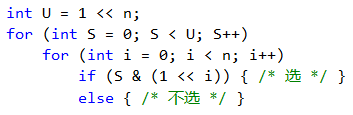
\includegraphics[scale=0.65]{pic/pic1.png}

	枚举两个集合,如果一个集合包含于另一个集合,
	那么它就是一个``子集的子集''。
	时间复杂度为 $O(4^n n)$。

	\subsection{子任务 2}

	枚举``子集的子集''的方法:

	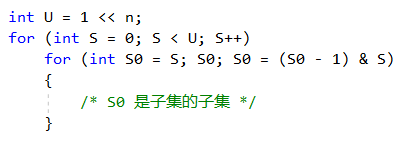
\includegraphics[scale=0.65]{pic/pic2.png}

	时间复杂度为 $O(3^n n)$。

	这东西紫书上是有的,你们都看了的吧。

	\subsection{子任务 3}

	全都是 $1$,这怎么做呢?

	现在问题实际上是问的\textbf{子集的子集的个数}。

	\textbf{考虑对答案的贡献。}
	我们先选出一个子集,把它视作一个``子集的子集'',
	再来看它包含于哪些子集中。
	显然,对于一个大小为 $k$ 的``子集的子集'',
	它被包含于 $2^{n - k}$ 个子集。
	因此对于一个大小为 $k$ 的子集,
	它作为子集的子集对答案的贡献为 $1 \times 2^{n - k}$。

	总共有 $\mathrm{C}_{n}^{k}$ 个大小为 $k$ 的子集,
	所以最终答案为:
	$$
	\mathrm{C}_{n}^{1} 2^{n - 1} +
	\mathrm{C}_{n}^{2} 2^{n - 2} + \cdots +
	\mathrm{C}_{n}^{n} 2^{0}
	$$

	由二项式定理,上式等于:
	$$
	\mathrm{C}_{n}^{0} 2^{n} +
	\mathrm{C}_{n}^{1} 2^{n - 1} +
	\mathrm{C}_{n}^{2} 2^{n - 2} + \cdots +
	\mathrm{C}_{n}^{n} 2^{0} -
	\mathrm{C}_{n}^{0} 2^{n}
	= (2 + 1)^n - 2^n
	$$

	什么你不会组合数?你不会二项式定理?
	趁其他人还没有在上数学课时学的时候偷偷学一波啊!
	当然,你会的话最好了。

	\subsection{子任务 4}

	还是考虑对答案的贡献。
	只要我们知道了所有大小为 $k$ 的子集的积的和,
	这道题就解决了。

	考虑动态规划。设 $f_{i, j}$ 表示在前 $i$ 数中
	选 $j$ 个数出来构成子集的积的和。
	边界条件为 $f_{i, 0} = 1$,最后要用的为 $f_{n, i}$,
	状态转移方程为:
	$$
	f_{i, j} = f_{i - 1, j} + a_i \times f_{i - 1, j - 1}
	$$

	最后的答案为:
	$$
	\sum_{i = 1}^{n} f_{n, i} \times 2^{n - i}
	$$

	时间复杂度为 $O(n^2)$,空间复杂度可以用滚动数组优化至 $O(n)$。

	显然子任务 4 要比子任务 3 简单,因为你不用二项式定理,也不用组合数,
	只用动态规划就是了。而且会做子任务 4 还能得到子任务 3 的分,划算吧。
	你敢说你没学过动态规划吗?

	\subsection{子任务 5}

	考虑生成函数。将每个数看作 $A_i(x) = 1 + a_i x$,
	则 $\prod_{i = 1}^n A_i$ 的 $i$ 次项系数就表示在 $n$ 个数中选 $i$ 个数
	它们的积的和。
	由于模数为 $998244353$,因此使用分治 NTT,在 $O(n \log^2 n)$
	的时间复杂度内求出子任务 4 里提到的 $f_{n, i}$。

	什么你不会生成函数?生成函数又叫母函数,
	你可以去缠着数学竞赛的同学问,叫他们讲懂为止[滑稽]。

	有问题就问数学竞赛的同学吧,谁叫``数学是人类进步的阶梯''呢?

	\subsection{线性算法}

	对于一个数,我们实际上可以认为它有 $3$ 种选择:
	
	\begin{enumerate}
		\item 它是子集的子集中的元素。

		\item 它是子集中的元素,但不是子集的子集中的元素。

		\item 它不是子集中的元素。
	\end{enumerate}

	考虑一个数对子集的子集的权值(简称权值)的贡献。
	对于第一种选择,它会让权值乘上 $a_i$;
	对于后两种情况,它会让权值乘上 $1$。
	
	对于下面这个式子:
	$$
	(1 + 1 + a_1)(1 + 1 + a_2) \cdots (1 + 1 + a_n)
	$$
	
	把它用多项式乘法的方法展开(先不要合并 $1$),对于展开后的每一项,
	正好就对应一种情况的权值。
	而这些项的和表示的就是所有情况的权值之和。

	现在把 $1$ 合并,上式变成:
	$$
	(2 + a_1)(2 + a_2) \cdots (2 + a_n)
	$$

	我们不允许子集或者子集的子集为空集,
	也就是说不能没有数选择 $a_i$。
	这就说明所有数都选择的 $2$,我们把答案减去 $2^n$ 即可。
	\subsection{实际得分情况}

	仅有一位同学得分 32,其余同学爆零。
	
	这位得分的同学的做法非常非常非常棒,它的做法的时间复杂度仅为 $O(2^n n)$,
	这是我没有想到的。

	方法是先枚举一个``子集'',
	再用 $O(n)$ 的方法计算出这个子集的子集对答案的贡献。

	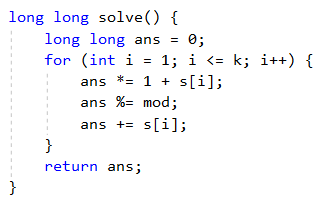
\includegraphics[scale=0.65]{pic/pic3.png}

	设 $f_{i}$ 表示在前 $i$ 数中任选数构成\textbf{非空}子集,
	它们的积的和。
	状态转移方程为:
	$$
	f_{i} = f_{i - 1} + f_{i - 1} \times a_i + a_i;
	$$

	状态转移方程中,第一项表示不选 $a_i$(但至少选一个),
	第二项表示选 $a_i$,但 $f_i$ 的定义使其表示的内容为
	``选 $a_i$ 的同时至少再选一个'',第三项表示只选 $a_i$。

	边界条件为 $f_{0} = 0$(没得选,又要求非空,那和就只能为 $0$ 了)。

	\subsection{做题总结}

	枚举子集,枚举子集的子集。
	
	考虑对答案的贡献。

	\section{T3:lyc 的农场(小 P 的牧场)}

	\subsection{写在前面}

	本来我是打算改了题面发 PDF 的,没想到你们在题库上做,
	但题库上的题面没有改,题的顺序也变了……

	半数以上的同学得到了满分,干得不错,那么我就不说怎么做了,
	你们可以讨论交流(逃

	不过斜率的英文是 slope,不是 slop,别背错了。

	\subsection{实际得分情况}

	仅有 4 名同学未得到满分,其中 3 名同学实现了 $O(n^2)$ 的暴力,
	很好。最后一位同学似乎 $O(n^2)$ 打炸了?

	\subsection{做题总结}

	一定要打暴力!打暴力不仅可以防止爆零,还能协助检查正解是否写错。

\end{document}